\documentclass[reprint,unsortedaddress,amsmath,amssymb,aps,prl,showkeys]{revtex4-2}
\usepackage{graphicx}% Include figure files
\usepackage{dcolumn}% Align table columns on decimal point
\usepackage{subfigure}
\usepackage{bookmark}
% \usepackage{biblatex}
\usepackage{float}
\usepackage{url}
\usepackage{bm}% bold math
\usepackage{hyperref}% add hypertext capabilities
\usepackage[mathlines]{lineno}% Enable numbering of text and display math

\begin{document}
\title{Role of Finite Allocation in Urban Development}
\author{Gezhi Xiu, Jianying Wang, Lei Dong}
\author{Yu Liu}
\email{liuyu@urban.pku.edu.cn}
\affiliation{Institute of Remote Sensing and Geographic Information Systems (IRSGIS), Peking University}
\date{\today}

\begin{abstract}
	Empirical evidence suggests that the evolution of urban systems is not only determined by local conditions, but also is constrained by regional status. We propose a out-of-equilibrium model of emerging cities within a given region, which explains the spatial transitions of development focus and urban shrinkage phenomenon in developed cities, while analytically keeping the classical results such as Clark's law for urban population density, and Zipf's law for cities' rank size distributions. We show that classical properties are only valid for cities within developing areas, and various urban diseases are inevitable given the limited regional resources. 
\end{abstract}

\maketitle

With all the advantages of modern cities in productivity and wealth creation\cite{Glaeser592,bettencourt2010unified}, we experience rapid population growth and accelerating demographic shifts to urban areas.%, which reaches a growing urbanization of 55\% people worldwide to live in cities. 
This brings an utmost importance of the interdisciplinary urban studies from a spatial complex systems perspective\cite{batty2007cities,batty2008size,portugali2011complexity,angel2005dynamics,boeing2017structure,PhysRevLett.79.523,bettencourt2013origins,batty2013new}. Specifically, models have been made on spatial shift to explain cities' morphology, and on migrations for global size distributions of area and population under equilibrium conditions. However, cities are dynamic, including not only temporal equilibrium attractiveness, but also globally organized restrictions from economical, political, and topographical conditions that lead to vicissitudinary development. To account for these aspects, we need a compelling generative model of emerging cities with systematic restricted conditions, with which we can deal with the fact that the attractiveness of urban areas is not eternal because of cities' marginal effect for latter stage of urbanization\cite{atkinson2012urban,girardin2009quantifying}.

While the forces behind vicissitudes of cities are complex, the advantages afforded by multi-scale densities of working population comprise an important driver\cite{smith1937wealth,fujita1999spatial}. Cities appear to be with higher density of working population, and support levels of enterprise impossible in villatic areas. More urbanized areas use resources more efficiently, resulting in more inventions and patents with fewer roads and supplies per capita\cite{fujita1999spatial,becker1999population,bettencourt2007growth}, meanwhile attracts more workers than less urbanized areas. The allocation of resources are operated by regional government to maximize productivity. At the early stage of urbanization process, emerged urban areas, fed by advanced techniques, totally outperform countrysides in economy and show high attractiveness to labors. However at the latter stage, the role of allocations matters more in spatial economy: constrained by the limited amount of labor and technical improvement, urbanization is controlled by a systematic cap. This is also reflected through urban sprawling, poly-centric transitions, and urban shrinkage, which convince us the avoidance of crowded urban centers and equilibrium. Existing models, however, usually set population density as the strength of attraction to new settlements\cite{PhysRevX.4.011008,PhysRevLett.79.523,foster2010communities,pan2013urban,Li2017Simple} to consequent on global Zipfian distribution of city population sizes\cite{zipf1949human}, where in a country, the largest city is about twice the size of the second, three times of the third, and so forth. Such setting contradicts with another universal observation that the agglomeration phenomenon includes economies and diseconomies of scale\cite{batty2019urbanscalinglaw}. The unsynchronized evolution of population and physical environments are keystone to understanding it\cite{doi:10.1177/0042098010396239,gu2001social}. Here, we present a stochastic growing model of urban systems, which relies on the assumption that agglomeration effects of infrastructures and population are separated. These principles guarantee more realistic predictions, such as urban core's spatial shift over time and urban shrinkage, while keeping vital properties such as Zipf's and Clark's law\cite{clark1951urban} of urban systems. 

To address the diseconomies phenomena in urban development, we need to adjust the setting of attractiveness, by redefining that as active, or working population, limited by current technology level or density of facilities. Recent developments shed some light on this concern with allocations of resources to enable systematic  growth\cite{schaigorodsky2018short}. The strength of attractiveness is determined by the local density. Coping with urban problems, we consider the a geographical setting that every establishment of site divides some space, and cities emerge uniformly over the given region. Once a city is established, it starts to grow with the speed of its partition of resource. This process turns into another phase of resource transference when the partition is finished, which is similar to realistic competition among cities and urban sites. Combining with spatial shifts of newly established sites, we encapsulate principles of a disequilibrium model to support long-term urban growth.


% Various attempts has been made to gain insight into mechanisms underlying complex features of cities about urban forms and scaling features. For instance, urban population dynamics is considered as spatial homogeneity with local population shifts\cite{PhysRevLett.79.523}, or social networks with spatial attaching\cite{PhysRevX.4.011008,pan2013urban}, or matching growth for individual\cite{Li2017Simple}. Existing models have succeeded in explaining regional emerging mechanisms of cities\cite{PhysRevLett.79.523} by reforming statistical laws and spatial patterns\cite{gabaix1999zipf's,clark1951urban}. The principles of such mechanisms lies in two parts, population settlement and economic growth, both of which changes spatially over time asynchronously. Traditional studies of spatial economics have attempted to construct this phenomenon under equilibrium models of regional urban systems\cite{batty1992form}. These models base their idea on agglomeration economies to explain why urban features, including population, tend to gather. However, cities are dynamical\cite{batty1971modelling}. The dynamics of spatial shifts between urban equilibrium (say, poly-centric transitions of cities), is poorly interpreted throughout these models. 
% First, %the initial states of 
% urban structures are assumed to be homogeneous, i.e., different urban aspects evolves synchronizedly and identically. However, urban constructions are in favor of fashion industries at different time, which shows that cities are out-of-equilibrium systems with unsynchronized growth driven by the interplay between infrastructure and population. 
% Second, these models mostly address city agglomeration's benefits by links\cite{Barabasi509}, standing for interaction between pairs of individuals. This brings difficulties in understanding the hierarchy and functional divisions that can be seen in nearly all cities\cite{bassolas2019hierarchical}. Thus we shall address attractiveness through other entities, e.g., the amount of public services. Meanwhile, separating the growth dynamics of infrastructures and population has not been taken serious attention, though some work in complex networks has realized that preferential attachment has hysteresis effect in setting up communication\cite{foster2010communities,hu2008urban}. 
% %%citation
% Lastly, throughout the abundant data describing cities, existing models cannot make quantitative predictions with more information added.% We present a stochastic growing model of urban systems, which relies on the assumption that agglomeration effects of infrastructures and population are separated. These principles leads to more realistic predictions such as urban core's spatial shift over time and urban shrinkage, while keeping vital properties of urban systems. 

%% 2019-12-18 添加,增加一段讨论城市收缩。
With the evolution of modern urban systems, cities suffer new dilemmas mainly resulted from constraints of space and crowdedness\cite{haase2014conceptualizing,martinez2012shrinking, PhysRevLett.120.108701,manoli2019magnitude}. These show that cities' free growth at a microscopic scale may results in an unsatisfactory global state, since agglomeration effects\cite{batty2013new} brings not only more innovations and productivity, but also congestion and friction. 
Such phenomena are hardly understood by existing models of cities, for preferential growth in all area leads to unbounded urban sizes, which is unrealistic for given social and natural conditions. To model cities with such concerns, we need to consider the individual sizes comparing with urban system. Thus we consider the \emph{active} part of population, who contributes mainly to urban construction and leads the up-coming population increase. Meanwhile, such group also corresponds to the maximum of urban supplement, over which can be regarded as exceeding region's economical or environmental limit. These people add up to the region's \emph{memory kernel}, serving as the constraint of the system's preferential growth\cite{PhysRevE.97.022132}.

Following the discrimination of growing preferences of population and infrastructures, we omit certain details and focus on the basic growth process over long time period by building a minimal model that replicates the basic properties of urban systems. Elaborately, since urban dynamics exhibits strong spatial auto-correlations (a city share the limited part of regional resources), we set up a partly-pure birth spatial model to account for the unforeseen cases both qualitatively and quantitatively. The model we propose is thus the essence of city mass evolution and regional vicissitude. We focus on newly joint population's attracting the force of infrastructure building, its impact on urban shrinkage in space and regional rank injection. 

% 微观角度如何构建模型,空间结构。

\begin{figure}
    \centering
    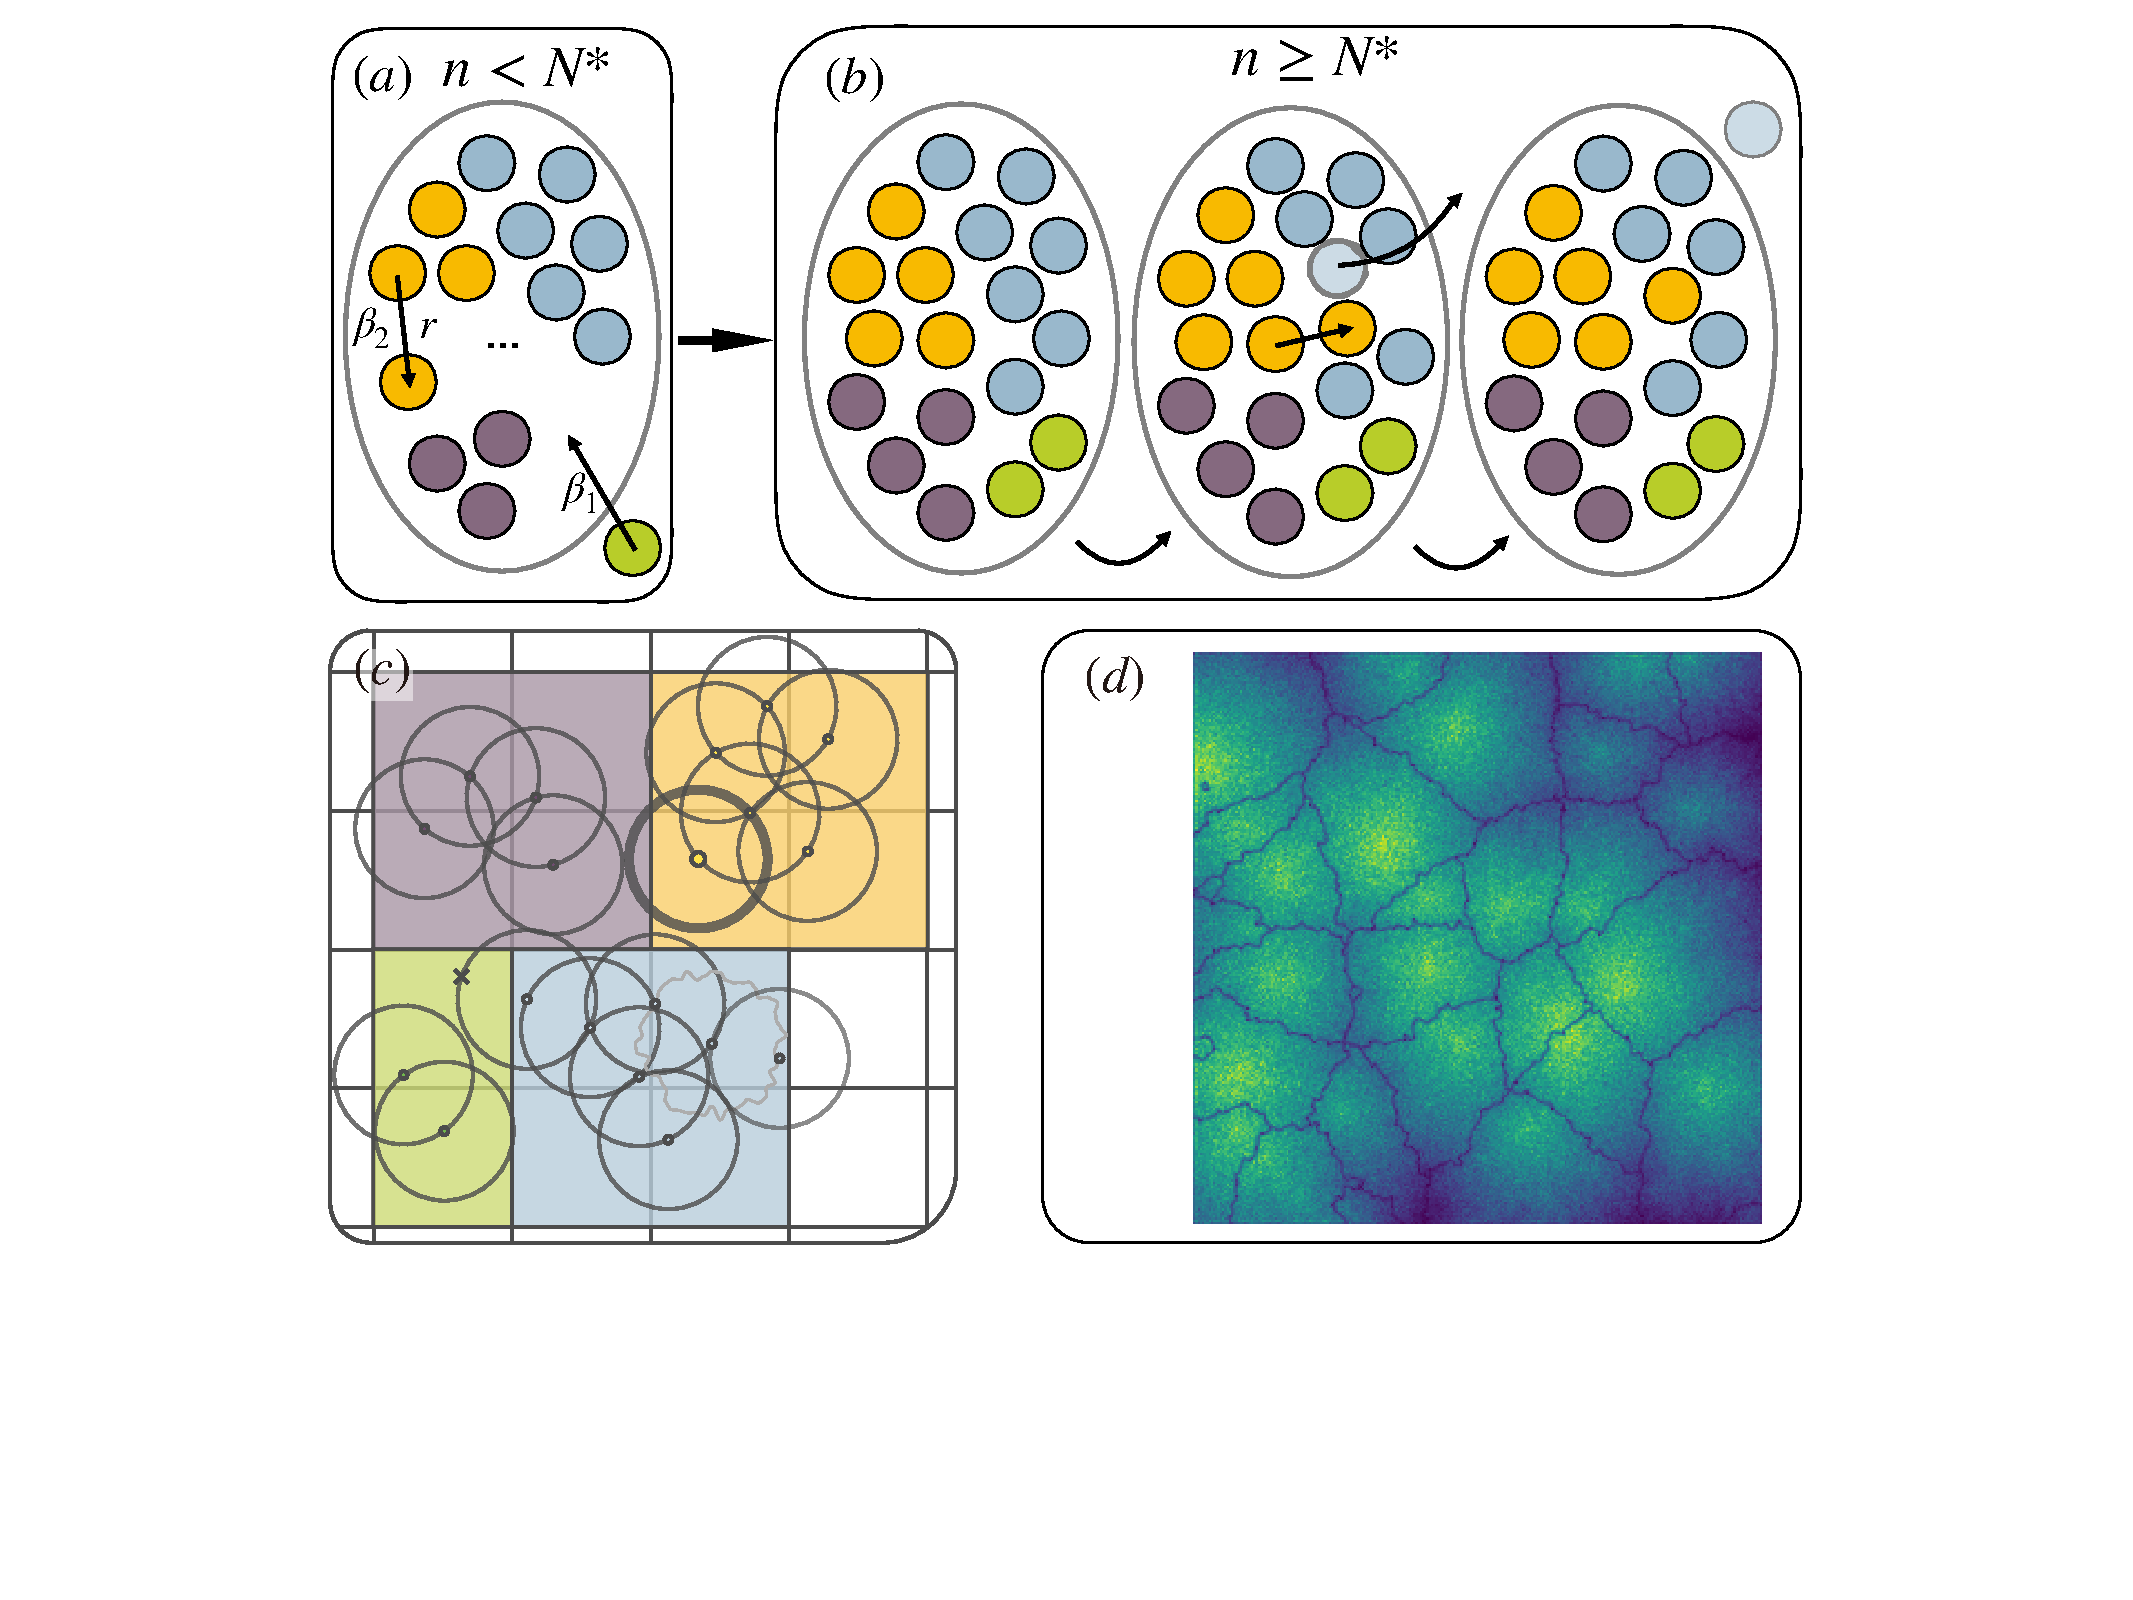
\includegraphics[width = 0.95\linewidth]{pics/sketchgood.pdf}
    \caption{(a) Status in the memory kernel at the first phase, where the total population $n$ is less than the size of the memory kernel, $N^*$. Existing nodes introduce new nodes at the rate $\beta_2$, while each existing city (noted by nodes in different colors) introduces new cities at the rate $\beta_1$. (b) When the memory kernel is fulfilled, every introduction of new city or node leads to an ejection of existing node currently included in the memory kernel. (c) The spatial aspect is that, an offspring node is landed at distance $r$ from the ancestral node. Also, when the kernel is filled, a new yellow node ejects an existed blue node, resulting in depriving its ability to introduce offsprings. (d) A simulated result for $L$, $r$, $\beta$ equals to $256$, $0.5$, and $4$, respectively.}
    \label{sketchpic}
\end{figure}

Our model describes how different cities (groups of individuals) grow spatially through attracting more individuals within a given area. As the model is based on geographical issues, a natural setting is a two-dimensional Euclidean space filled with nodes denoted by the coordinates in $\mathbb{R}^2$ on an $L\times L$ square. If an attracted individual is placed on an empty block, this block becomes the possession of the individual's city, i.e., latter individuals introduced by other cities cannot survive on such block. This model can thus be regarded as the process of urbanization on individual level. We denote a meta-population, i.e., a person or a small group of homogeneous people, as a node, which is labeled with the unique city it belongs to. People either establish new cities, or join existing cities. We assume that either process proceeds at a constant rate, that is, the frequency of forming new cities is proportional to the number of existing cities; And the number of newly joint nodes of each city is proportional to its population. We denote the two relative speeds as $\beta_1$ and $\beta_2$. These settings are parallel to Yule's original model\cite{yule1925ii}\footnote{Yule model is originally based on the observation of older genus and species tend to have existed longer}. These settings lead to exponential waiting times for a city or a node to attract a kin into the system, which also conform to urban systems under stable socio-economic conditions. 

The spatial aspects are stated as follows. New cities emerge continuously and uniformly over the considered area, as a Poisson point process\cite{miles1970homogeneous}. An emergence is confirmed is its location belongs to some untaken block. In every emerged city, a newly joint node is \emph{introduced} by an existing node, located at a distance of $r$ near the existing one of some random direction $\theta$. We take $r < 1$ to make sure that new comer is located at or at the neighbor of the introducer's block. In global perspective, cities' growing process is like a diffusion process\cite{RevModPhys.87.925} with some seed points sprinkled on the area as blocks are gradually carved up into the regime of growing cities. We name this process as \emph{Spatial Yule Model (SYM)}.

As we can see, blocks with more nodes have higher probability to introduce new people nearby. Such natural formation of urban systems resembles the population distribution in emergence of many regional systems with adjustable parameters. However, regional growth also faces difficulties of economical bottlenecks and the need of balancing regional growths. In the meantime, the regional authority can only invest finite resource in infrastructure construction. These facts imply that we have to add a limit on growing process to reflect the truth. Thus we introduce a \emph{memory kernel}. Memory kernel denotes a list of nodes that are able to introduce new nodes into the system. We name it so to cater the finite size effect, a  It can be interpreted by the following statement: New comers needs supply to settle, thus he carries a \emph{coin} to get her settled. However, the total regional resource is limited that the amount of coins is limited, say $N^*$. So from the $(N^*+1)$'th person that settles in a city of this region, she carries a coin as a pre-comer loses hers. Thus when the regional fortune has all been shared, all money is only transferred to the new comers, to allow their essential needs of infrastructures. A sketch map for the whole model is shown in Fig.\@\ref{sketchpic}.

%%%%%%%%%%%%%ckpt
We now discuss the variables $\beta:=\beta_1/\beta_2$. The problem of determining the relative speed of city's generation is very reminiscent of some problems encountered in gas physics. It is interesting to investigate the number of cities in a given regions of the same population. Some groups tend to form new cities to have sufficient infrastructures and less diversity of urban output ($\beta > 1$) and some cities may go otherwise ($\beta< 1$). This value is actually a reflection of the intensity of regional industry. On the other hand, smaller $\beta$ can be interpreted as smaller studied area. Speaking of $r$, the metropolis areas over the world have very different densities. In SYM, it determines the sprawl of a city with given population. It can also be taken as the area proportion for a city in the studied region. On the other hand, it is also constraint of regional growth controlling the expected allowance of cities. % We take $r=1/2$ as default for simulations.

Regarding the size of the memory kernel, $N^*$, we realize that it is related to the authority's financial ability to supporte more incomer of the region. The competition of resource is neglectable if population is few. As it grows, cities's infrastructure constructions mostly supply those who are contributory for urban economics. In our framework, we choose the hard kernel with a fixed size, so that the economic process can be captured by the partition of coins in different study areas, say, cities or blocks. More coins distributed in a city leads to more attraction to future residents, the case is the same for blocks. Limited resource leads to resource allocation and regional economy, which changes spatially over time. 

In summary, our model is defined under three parameters, $\beta$, $r$, and $N^*$. In every exponential time (before the memory kernel is filled), an existing node introduces a new node located from $(r,\theta)$ of her. Meanwhile a new city is introduced by an existing city in another exponential time at somewhere empty. So that the urban system is growing acceleratingly at the first phase, during which every individual owns a coin with her. In the second phase, the memory kernel is full, i.e., the total population exceeds $N^*$, only those who own coins (sum up to $N^*$) can introduce new comers in the future. Existing ones will stop introducing sometime almost surely. We denote the population of a city $i$ at time $t$ as $N_i(t)$. The master equations for the first state when the memory kernel is underfull is \[\frac{\partial}{\partial t}N_i(t) =  \delta_{N_i(t)}\cdot k\beta_1+ (1-\delta_{N_i(t)})\cdot N\beta_2, \]while the master equations for the second phase goes to
\begin{align}
    \frac{\partial N_i(t)}{\partial t}  = (N^*\beta_2)[\frac{N_i(t)}{N^*}\cdot(1-\frac{N_i(t)}{N^*-1})& \notag\\  - (1-\frac{N_i(t)}{N^*})\cdot (1-\frac{N_i(t)}{N^*-1}) ]&
\end{align}
% \begin{align}
%     P(N_i(t_{n+1}) = N_i(t_{n})+1) &= \delta_{N_i(t_n)}\cdot\frac{k/\beta_1}{k/\beta_1 + n/\beta_2}\notag \\ &+ \frac{n/\beta_2}{k/\beta_1 + n/\beta_2}\frac{N_i(t_{n})}{\sum_i N_i(t_{n})} \notag \\
%     P(N_i(t_{n+1}) = N_i(t_{n})) &= \frac{k/\beta_1}{k/\beta_1 + n/\beta_2}\notag \\ + \frac{n/\beta_2}{k/\beta_1 + n/\beta_2}&\cdot (1-\frac{N_i(t_{n})}{\sum_i N_i(t_{n})}),
% \end{align}
% while the master equations for the second phase goes to\begin{align}
%     &P(N_i(t_{n+1}) = N_i(t_{n})+1)=\frac{i}{N^*}\left(1-\frac{i}{N^*-1}\right)\notag\\
%     & P(N_i(t_{n+1}) = N_i(t_{n})-1)=\left(1-\frac{i}{N^*}\right) \cdot \frac{i}{N^*-1}\notag\\
%     & P(N_i(t_{n+1}) = N_i(t_{n}))=\left(1-\frac{i}{N^*}\right) \cdot\left(1-\frac{i}{N-1}\right) \notag\\ &\hspace{5cm}+ \frac{i}{N}\cdot\frac{i}{N-1}.
% \end{align}
And the direct corollary is that $P(N_i(\infty))$ will converge to $0$ or $1$ almost surely since the memory kernel is fulfilled. 

% Cities are places that concentrate human innovations and productivities. It has been well studied that urban output grows as fast as urban sizes. This results in some interesting results of urban studies on various scales. For inner-city properties, the classical common knowledge is that the population density decay exponentially from core to periphery; As well as cross-city level, the rank size distribution of cities, known as Zipf's law, is the indicator for how much more attractive a bigger city is than smaller cities. These findings are keys to understanding urban formation patterns. In recent years, researchers in urban studies are devoted to reformulate complex cities with simple rules. 

% While our interest lies in hte spatial distribution of population, there are other feathers of urban growth for which parallels with economical development over geographical space can be drawn, for mathematical methods applied. For example, the rank-frequency distribution of urban population\cite{gabaix1999zipf's}, can be explained using a novel form of the Yule process, first introduced to explain the distribution of the number of species

Depending on the relative importance of city sprawl, emergence rate, and economic constraints, SYM predicts the existence of three phases: freely growth phase, economic constraint phase, and spatial constraint phase. We focus on the first two phases above, that correspond with cities' memory. From now on, we will assume that $N^*$ and $L$ are large enough so that the free growth phase exists for small population. In such phase, cities grow desolately, without being controlled by total resource and space. We now describe two important properties of this phase, stately (1) Zipf's law\cite{gabaix1999zipf's} for rank size distribution of cities' population, and (2) Clark's law for mono-centric cities' population density. 

%%%%%%%%%%%%%%%%%%%%%%%%%%%%%%%%%%%%%%%%%%%%%%%%%%%%%%%%
The populations of cities typically decay proportionally to the inverse of their ranks\cite{gabaix1999zipf's}. This is referred as Zipf's law of cities' population sizes, i.e., the populations of cities distribute as a power of ranks, $f_r(r)\sim r^{-(1+\beta)}$. Recall that the number of individuals in the system at time $t$, $N_i(t)$, has a geometric distribution\cite{durrett1999essentials}, $P(N_i(t)=n)=e^{-\beta_1t}(1-\exp(- {\beta_1} t))^{n-1}$, and the second assumption that the number of cities will grow exponentially at rate $k\beta_1$, if we pick a random city, the time since its first appearance will have an exponential distribution of $\beta_1$. Thus the distribution of the population of a random city is 
\begin{align}
	f(n)=\frac{\Gamma(1+1/\beta)\Gamma(n)}{\beta\Gamma(n+1+1/\beta)}\approx Cn^{-1-1/\beta}, \ \text{as } n\rightarrow\infty,
\end{align}
where $\Gamma(\cdot)$ is the gamma function. This implies a Zipf's relationshio with $n(\text{rank})\sim {rank}^{-\beta}$. Noticing that $\beta$ takes value from all positive real number in SYM, we can derive arbitrary scaling behaviors by switching $\beta$. According to some existing studies\cite{PhysRevLett.79.523}, the power law dependence of population frequency is $2.03\pm 0.05$ for the world, indicating the average relative emerging rate of cities is around $1.03$. The experiments have confirmed our analytic results for the first phase in SYM. A simulated validation for this result can be reflected in Fig.\@\ref{fig:rankditribution}. 
\begin{figure}[t]
    \centering
    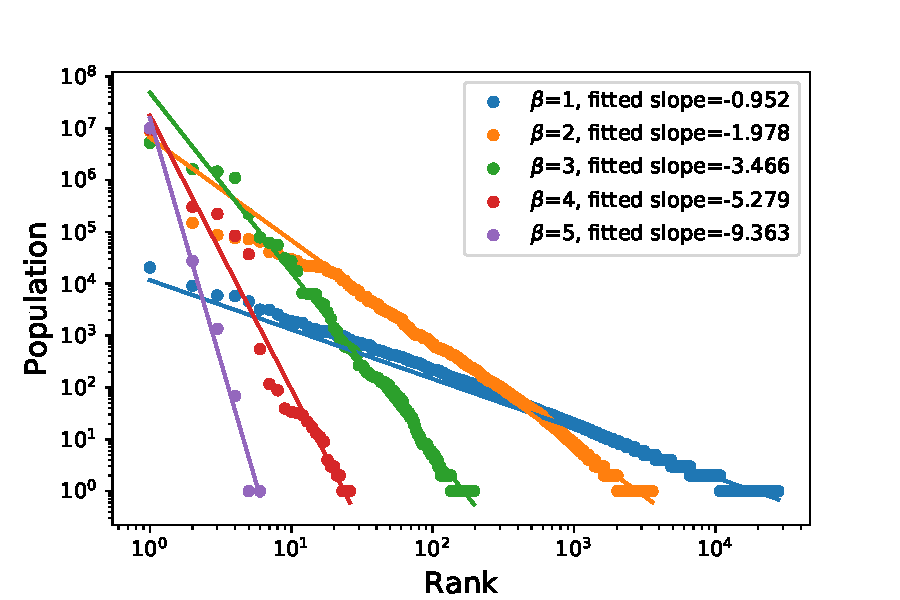
\includegraphics[width=0.48\textwidth]{pics/zipf.pdf}
    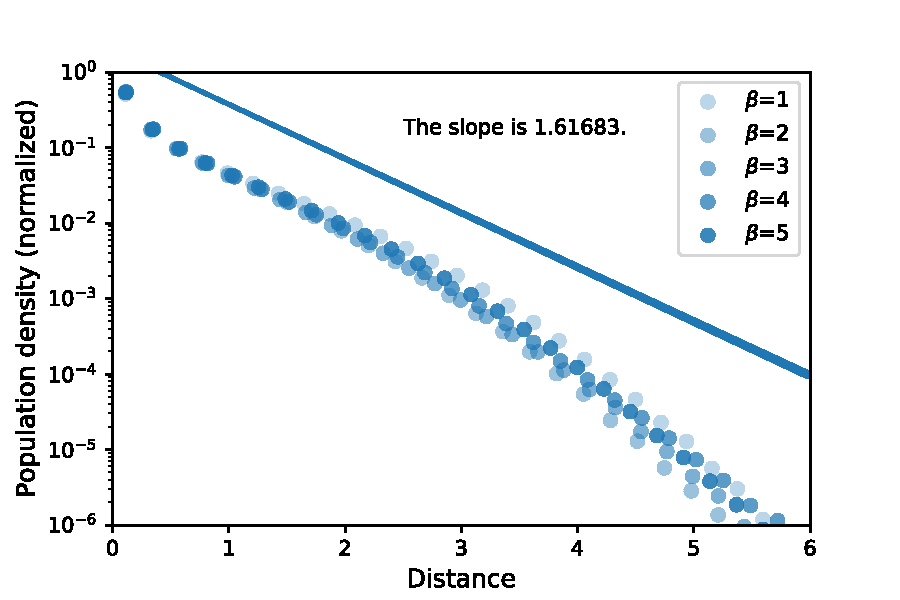
\includegraphics[width=0.48\textwidth]{pics/kernal_density.pdf}
    \caption{(a) The distribution of population among communities. In the simulation we take $N = 10^5$, $\beta_2=1$ and $\beta_1 = 2$. The theoretical prediction of the slope is $-1.5$, and is well approximated by the simulated results. This result confirms that Zipf's law is valid for growing urban systems where all cities share the same rate to grow. From the other master equation we analyze that this observation vanishes if total growing force is limited. (b) The population distribution as a function of distance from a district's center. The vertical axis is logarithmic processed, which represents the exponential decaying of population distribution. Regardless of the finite-sample effect, we fit the middle part of population density's spatial distribution to the exponential distribution with a slope of $-0.95$, which approximately equals to $1-1/\beta$. This fit has a confidential measurement of $R^2=0.99$.}
    \label{fig:rankditribution}
    \label{fig:clark}
\end{figure}


% }

% \subfigure[]{
%     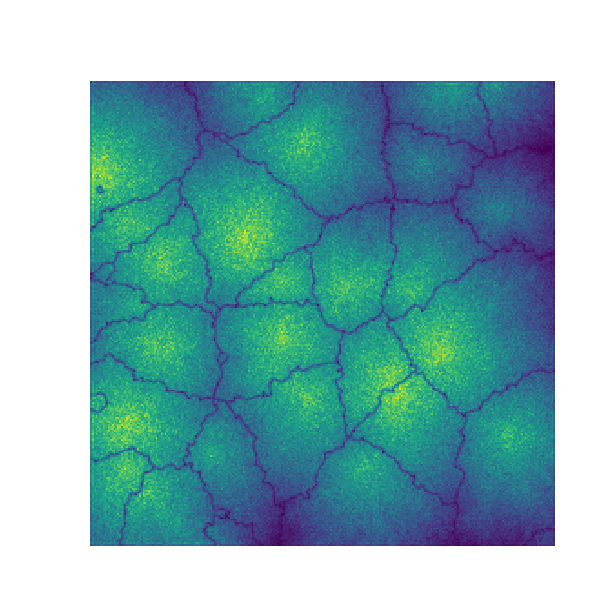
\includegraphics[width=0.3\textwidth]{pics/fractal_41_256.pdf}
%     \label{fig:fractal}
% }

% Adding these facts about area and population distributions, we confirmed the power law scaling behavior between them. This result confirms that the occurrence of universal scaling can be resulted by homogeneous local growth. Noticeably, this result only copes with the case when the space is sufficiently large, so that the population with spatial competition (edging block residents) is small. Simulation confirms our prediction as the slope of log-log plot turns to a flatter phase when population is too large. This can be interpret as the congestion effect, since the competition among cities affects more on larger cities as they control longer boundaries.

%% clark

Population density evolves as two-dimensional diffusion within a city\cite{doi:10.1137/0150099}, where we can focus the density's growth on each axis from the oldest nodes of a city. Let $\rho(d)$ denote the node density of places of the distance $d$ from a city's center, and $t_n$ as the time for the $n$'th node to generate, we have 
\begin{align}
    \rho_{t_{n+1}}(d) = (\rho_{t_{n}}(d-r) + \rho_{t_{n}}(d+r) )/2.\label{loc_den}  
\end{align} By re-scaling time as $\tau_n = t_n\cdot (k\beta_1+N\beta_2)/T$, for a sufficient large $T$, this equation\@s\ref{loc_den} results in a exponential decay of density
    \begin{align}
        \rho(d)\sim e^{-\alpha d}\label{clark_eq}.
    \end{align}
This is a reinvention of Clark's law in empirical urban studies\cite{clark1951urban}. Beyond solitary growth, we analyze the competitiveness of land for different cities. The population within an edging block of city $j$ is estimated by $e^{(T-T_j)}\int_{d}^{d+1}\rho(r)dr/(2\pi d)$, where $T_j$ is the emerging time of city $j$. We also have the waiting time $T_{n+1}-T_{n}\sim 1/n$, and the total population approximation $e^{\beta_1+\beta_2}$, combining which we derive the population of edging blocks if time and the urban radius are given. Since the attractiveness of large urban center is larger, the edging population of large cities is actually smaller than minor cities. We validate our prediction with simulations in Fig.\@\ref{fig:clark} %We give a detailed derivation in Appendix B\ref{edge_comp}.

% \begin{figure}
%     \centering
%     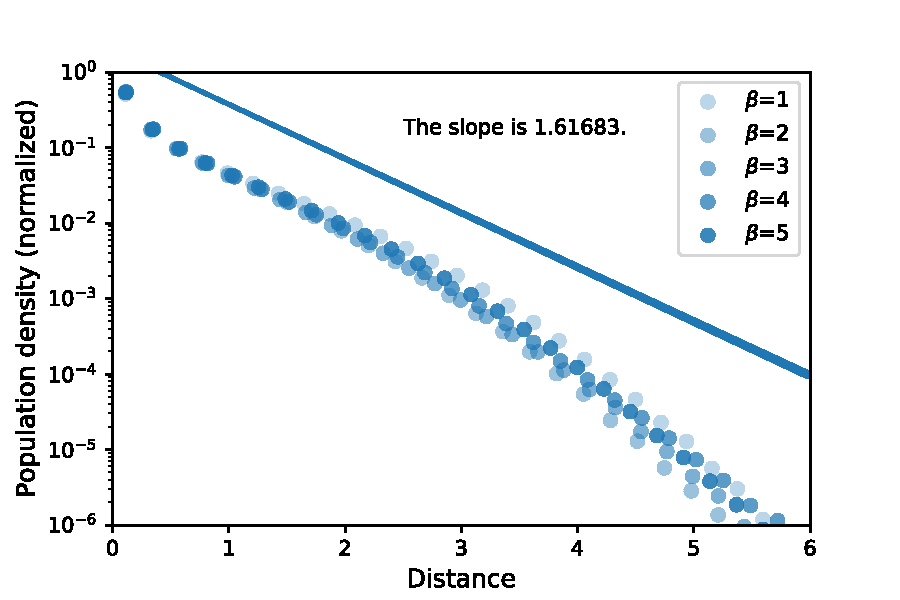
\includegraphics[width=0.48\textwidth]{pics/kernal_density.pdf}
%     \caption{The population distribution as a function of distance from a district's center. The vertical axis is logarithmic processed, which represents the exponential decaying of population distribution. Regardless of the finite-sample effect, we fit the middle part of population density's spatial distribution to the exponential distribution with a slope of $-0.95$, which approximately equals to $1-1/\beta$. This fit has a confidential measurement of $R^2=0.99$.}
%     \label{fig:clark}
% \end{figure}

%% mk  
The multi-dimensional coincidence between the exponents derived in our model and the universal exponents in empirical data of population distribution indicates that only two observation scales lead to the global behaviors of regional dynamics. This means that the actual urban growth has not yet reached the constrained cases. However, preventive measures are still necessary. Thus we bring a general constraining parameter $N^*$ to further discuss the second phase of SYM, the resource constrained phase, i.e., the total population reaches $N^*$, the size of memory kernel. Such setting is the abstract of many real-life rules set by global organizations such as the allowance of carbon emissions or sustainable development projects. In each city, a proportion of population are coin holders, labeled as memorized. Here, $\sum_{i=1} m_i(t) = N^*$ for $t$ that is sufficiently large. If in some period, the minor cities generate more offspring than major ones and the superiority of remaining population within the memory kernel changes, minor city will increase its ranking, as the growing rate for each city $i$ is actually $m_i\beta_2$. On the dynamics within the memory kernel, for each city, $m_i$ acts as a random walk with absorption wall $0$, since no offspring will be expected if no nodes are left in the kernel. This result also works for single block case within a city. Denote the population with a block $j$ of city $i$ as $m_{ij}$. According to\@\cite{durrett1999essentials}, we use a result for branching process that a block loses its vitality if the population goes downhill under a threshold \begin{align}\rho_{threshold} = k\beta_1/(2\beta_2)+N^*/2.\end{align} This value shall be regarded as the sign for \emph{urban shrinkage}, for the edging blocks have lower density according to equation\@\ref{clark_eq} thus have an exponentially higher probability to be languished. In other words, urban shrinkage shall be reasoned by limited systematic resources in the given region. 

The kernel mechanism also plays a role at the cross-city scale: The preference of larger cities is easier to fail. The competition for coins in SYM receives more than pure birth settings because the sum of fortune is given as $N^*$. In other words, SYM system doesn't suffer from inflation. To test this interpretation, we analyze the superior switching rate, defined as the average frequency of timesteps in a realization that the second largest city surpasses the largest in active population within the memory kernel. We conduct numerical experiments, and receive power law dependence between the frequency and the simulating steps, shown in Fig.\@\ref{changerate}. Moreover, the switching is more likely to happen with a memory kernal, i.e., switching with memory kernel decay slower in probability. It is also a clear result since a growing society (a society without a memory kernel) suffer less from interspecific competition.

\begin{figure}
    \centering
    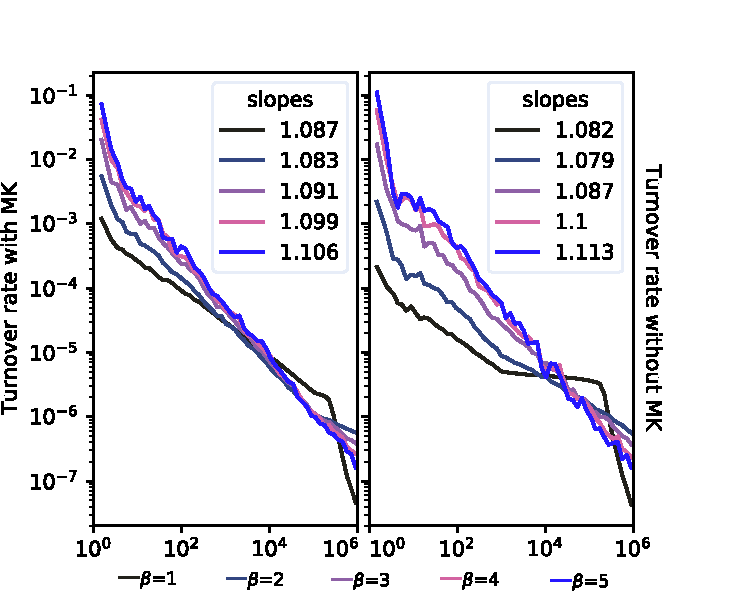
\includegraphics[width = 0.48\textwidth]{pics/in_one_now-10.pdf}
    \caption{The change rate statistics with and without a memory kernel. The kernal keeps the turning over more often. With same $\beta$'s, a kernel-based SYM's decay in turnover rate is smaller. These results validate our prediction that with finite resource, advantages are more likely to be kept.}
    \label{changerate}
\end{figure}

The last property of SYM is the fractality of urban envelop, stately, the length of urban edges vary with the used measurement. Inspired by multi-player interaction in fractal financial market\cite{PhysRevE.65.037106}, we interpret that fractal urban boundary is driven by the competition for land at cities' edges. In SYM, the uncertain competition for space lies in parameter $r$. A larger $r$ indicates larger randomness and brings an extra advantage for minor cities, resulting in a larger fractal dimension. We apply the box counting technique to calculate the fractal dimension of urban envelops, and receive an stable output of $d_f = 1.2\pm 0.05$ with $r = 0.5$, similar to empirical results\cite{batty1992form}. We also find larger $d_f$'s for greater $r$. These results validate our hypothesis that fractal edges coexist with spatial competition. 

%% Discussion

This \emph{Letter} concludes the urban system dynamics in only three key components, and receives fruitful results. Not only do SYM explain existing properties, such as Zipf's and Clark's law, but also predict regional trends in a probabilistic perspective. We analytically derive 
%the inter- and intra-city properties 
Zipf's law of global population, Clark's law for urban density, and the fractal behaviors of urban edges. Due to the simplicity of SYM, we investigate the future phase transition of urban development in great detail. The present results are derived two assumptions: (i) the stationary growth of individuals as parameters are all set to be constant and (ii) the limited resource can be equally treated as a partition of memory kernel. In practice, these assumptions are well-held if sufficient divergence of meta-population across the world is considered. In other words, the identification of a town is 30,000 in Japan, and 200 in Sweden, leading to different considerations of meta-population. Simulations of this model can be adjust to heterogeneous geographical circumstances by applying the growing rate on each block to the product of inherent dynamic $m_{ij}\cdot \beta_2$ and the local characteristic $c_{ij}$ to better suit for realistic conditions. The parameter $r$ best determines the type of metropolis over the world for identifying morphology of major cities. Central European cities share lower $r$, making the cities disjoint and centralized; while São Paulo metropolitan area indicates a larger individual preference for urban expansion. Although our results are not all analytically proved, we believe it is a essential step to strip out the power of urban dynamics. The model is non-commuting, but the community structure is naturally embedded. For further consideration, we can extend the model by adding links as the volume of exploration and preferential return between cities\cite{WANG2019121921}.

The memory kernel mechanism leads to a straightforward corollary that the construction of infrastructure is the reason of population's spatial transitions, as only those who are recorded in the kernel are considered as productive people that attract new-comers to his city. This result provides a bottom-up explanation of transition of urban centers with stochastic spatial shifts of cities' memorized people. It also tells that the economic growth is the basis of growth potentials. Under the circumstances of preferential attraction, if the size of the memory kernel cannot grow fast enough to match with population, the concentration of production will go far from tolerance. Taking the productive aspect together in the memory kernel helps to talk about many other properties like the age structure. The stationary age can be calculated as the average time for a new city to emerge is $(\beta_2 N + \beta_1 k)^{-1}$, which equals to the average losing age of the whole kernel. The model can further be extended with multi-dimensional memory kernel, allowing one node to emerge if different factors (i.e., the existing nodes in different dimension of kernel) coevolute to allow new nodes to emerge.% In words, the memory kernel mechanisms is fundamental.
\bibliographystyle{unsrt}
\bibliography{refs.bib}
\end{document}
